\null\newpage
<<<<<<< HEAD
\section{Tieftöner- und Hochtönerweiche}\label{sec:4.2}
\subsection{Allgemeines}\label{subsec:4.2.1}
Für die Satellitenlautsprecher, welche aus einem Hochtöner und einem Tieftöner bestehen werden nun die Teilfrequenzbereiche Mitte und Hoch benötigt. Da es sich bei dem Satellitensystem um ein Paar an Boxen handelt und diese räumlichen weiter entfernt voneinander stehen, können nun Stereo-Effekte verwendet und mit dem reinen Stereo-Eingangssignal gearbeitet werden. Eine Aufteilung des Signals in Linke- und Rechte-Satellitenbox muss jedoch schon getroffen werden, um die Effekte richtig zu erhalten. Dafür wird einfach für die Linke-Satellitenbox, bestehend aus Hoch- und Tieftöner die entsprechenden Weichen verwendet und das Selbe für die Rechte-Box.
=======
\section{Tieftöner- und Hochtönerweiche}\label{sec:5.2}
\subsection{Allgemeines}\label{subsec:5.2.1}
Die Satellitenlautsprecher (Kap. \ref{3.4}) bestehen aus einem Hochtöner und einem Tieftöner. Aus diesem Grund sind die Audio-Teilfrequenzbereiche Mitte und Hoch interessant. Dafür wird  für jede Satellitenbox jeweils eine eigene Hochpass- und Bandpass-Weiche verwendet. Effekt der jeweiligen Filter siehe Kapitel \ref{3.3}\\
Die  Ansteuerung der Satellitenboxen ist eine Aktive-Mono-Bass-Box, welche diese mit Signal versorgt. 
>>>>>>> origin/master

\subsection{Zielsetzung}\label{subsec:4.2.2}
Das unberührte Eingangssignal soll so gefiltert werden, dass der Hochtöner nur Frequenzen über 1,5kHz und der Tieftöner Frequenzen bis 6kHz zum abstrahlen erhält. Dementsprechend sollen die Filter gewählt und designet werden.\\
Obwohl es den Mono-Bass gibt der die untersten Frequenzen (>20Hz) abzustrahlen hat, dürfen die Satelliten-Tieftöner im selbigen Bereich ebenfalls spielen. Somit wird die abstrahlende Fläche vergrößert und freiwerdende absolute Pegel höher. Bei dem Satelliten-Tieftöner wird jedoch ein Bandpass vorgesehen um bei möglichen Resonanzen mit dem Mono-Bass das Signal filtern zu können.\\
Dementsprechend sollen die Filter gewählt und designet werden.

\subsection{Schaltung}\label{subsec:4.2.4}

Das Eingangssignal (Links, Rechts, Masse) wird an einer dreipoligen Stifleiste angeschlosssen (Abb. \ref{fig:4.2.4.1}). Zuerst gelangt Signal-Links und -Rechts an jeweils ein Potentiometer um den Pegel anpassen zu können, es bietet also eine Regelmöglichkeit. Es folgen die Filter. Hochpass für Links/Rechts und Tiefpass für Links/Rechts. Ein \enquote{Butterworth-Tiefpass-Filter 2. Ordnung} wurde bereits in dem Kapitel \ref{subsec:4.1.4} erklärt. Das \enquote{Butterworth-Hochpass-Filter und -Bandpass-Filter 2. Ordnung} weist keine groben Unterschiede auf, der Unterschied liegt lediglich in der Bauteilaufteilung.\\
Nach den Filtern gelangen die getrennten Signale zu deren Ausgangspunkt. Es ist für jede Signalleitung eine zweipolige Stiftleist vorgesehen (Signal + Masse), da der darauffolgende Verstärker einen selbigen Eingang besitzt. Die Stiftleisten sind jedoch gruppiert nach Bandpass- und Hochpass-Ausgang.\\
\begin{figure} [H]
	\centering	
	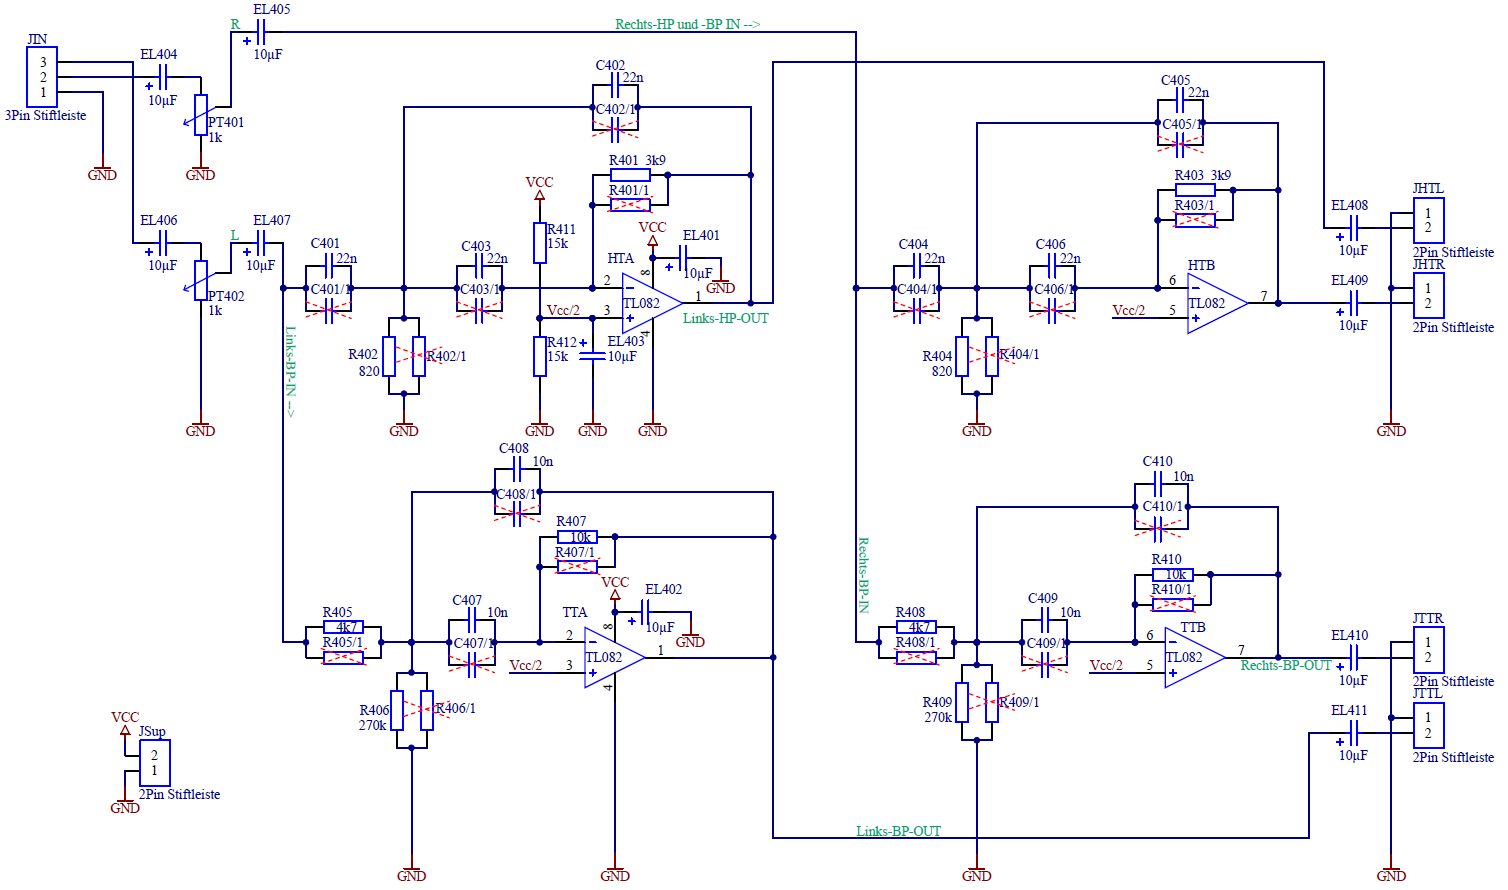
\includegraphics[width=1\textwidth]{img/Print4/4_TTuHTWeiche-Schematic.PNG}
	\caption{Butterworth-Bandpass-Filter 2. Ordnung}
	\label {fig:4.2.4.1}
\end{figure}
Eines der Bandpass-Filter. Gut sichtbar die doppelte, parallele Ausführung von Widerständen und Kondensatoren um krumme Werte auch erhalten zu können. Bedingt durch Parallel-Schaltung von Widerständen und Kondensatoren.\\ 
Der Eingang wurde gespiegelt um ein schöneres Bild zu erlangen. Die Spiegelung ist für das PCB-Layout nicht relevant!\\
Bedingt durch die Versorgungsspannung ist auch der Spannungsteiler für $\frac{Vcc}{2}$ am Plus-Eingang des OPVs implementiert.
\begin{figure} [H]
	\centering	
	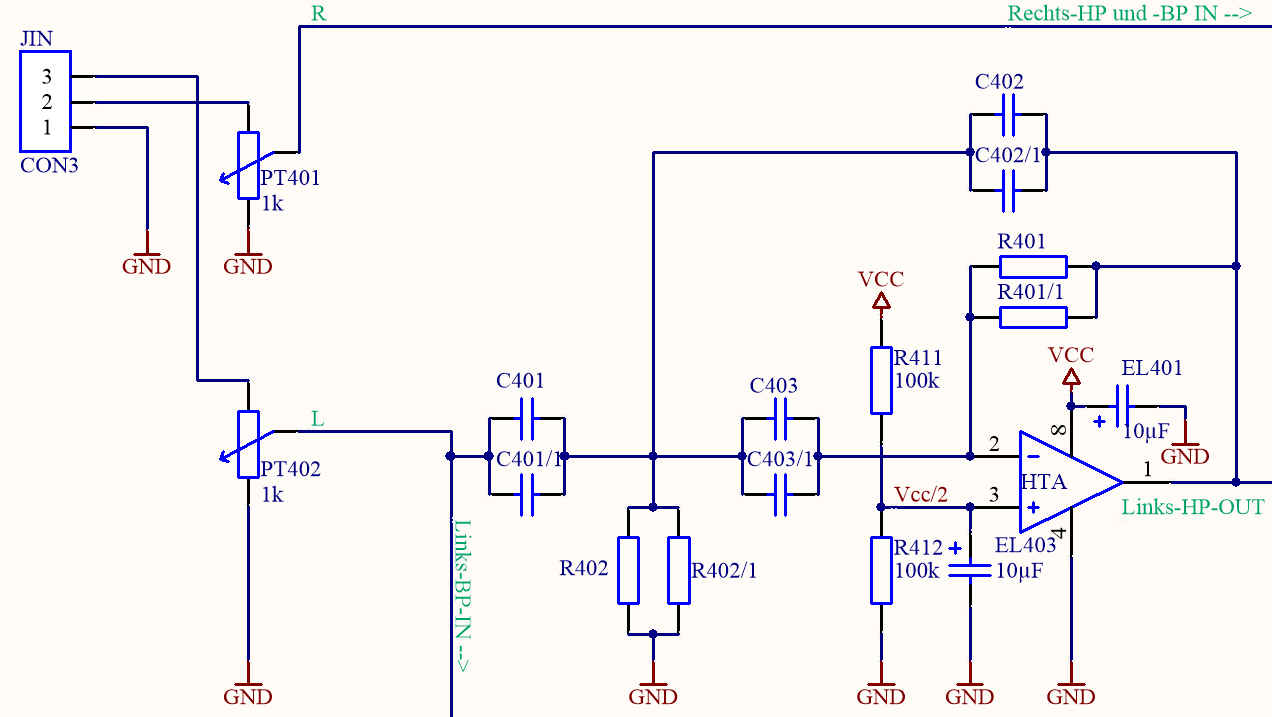
\includegraphics[width=1\textwidth]{img/Print4/4_TTuHTWeiche-LinksHP-Schematic.PNG}
	\caption{Butterworth-Bandpass-Filter 2. Ordnung - aus Abb.\ref{fig:4.2.4.1}}
	\label {fig:4.2.4.2}
\end{figure}
Am B-Teil des OPVs (erkennbar an der Beschriftung: TT\enquote{B}) ist keine Versorgung einzuzeichnen, da er mit dem A-Teil einen achtpinnigen IC mit zwei integrierten OPVs ergibt. Die zwei Teile sind über das IC-Gehäuse mit der gleichen Versorgungsspannung verbunden, deshalb ist das einmalige Kennzeichnen ausreichend.\\
\begin{figure} [H]
	\centering	
	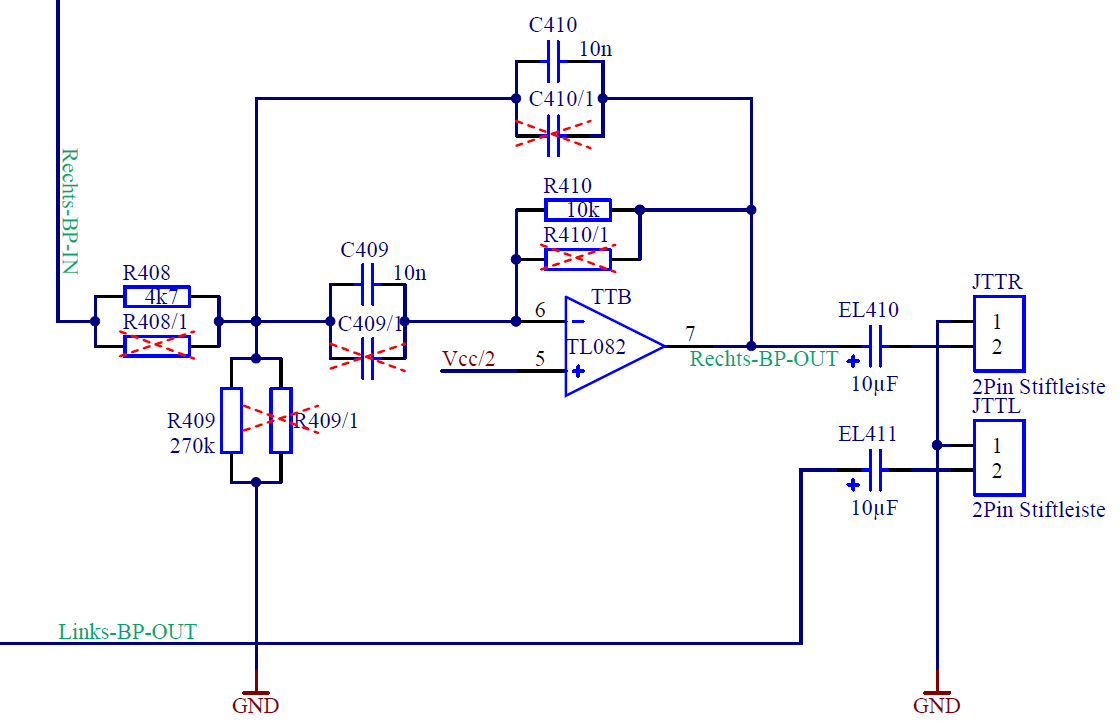
\includegraphics[width=1\textwidth]{img/Print4/4_TTuHTWeiche-RechtsBP-Schematic.PNG}
	\caption{Butterworth-Bandpass-Filter 2. Ordnung - aus Abb.\ref{fig:4.2.4.1}}
	\label {fig:4.2.4.3}
\end{figure}

<<<<<<< HEAD
\subsection{PCB}\label{subsec:4.2.5}
Es wurden die grundlegenden Regeln zur Leiterplattenentflechtung angewandt (\ref{subsec:3.1.2}). Bei dem Design (Abb. \ref{fig:4.2.5.1}) wurde auf hohe Variierbarkeit geachtet um auch zB. Kondensatoren mit unterschiedlichen Footprint verwenden zu können.\\
=======
\subsection{PCB}\label{subsec:5.2.5}
Es wurden die grundlegenden Regeln zur Leiterplattenentflechtung angewandt (\ref{subsec:3.1.2}). Bei dem Design (Abb. \ref{fig:5.2.5.1}) wurde auf hohe Variierbarkeit geachtet um auch zB. Kondensatoren mit unterschiedlichen Footprint verwenden zu können.\\
>>>>>>> origin/master
Es wurden wieder nahe an den IC's ELKOs in der Spannungsversorgungsleitung verbaut, um Störungen zu verhindern.

\begin{figure} [H]
	\centering	
	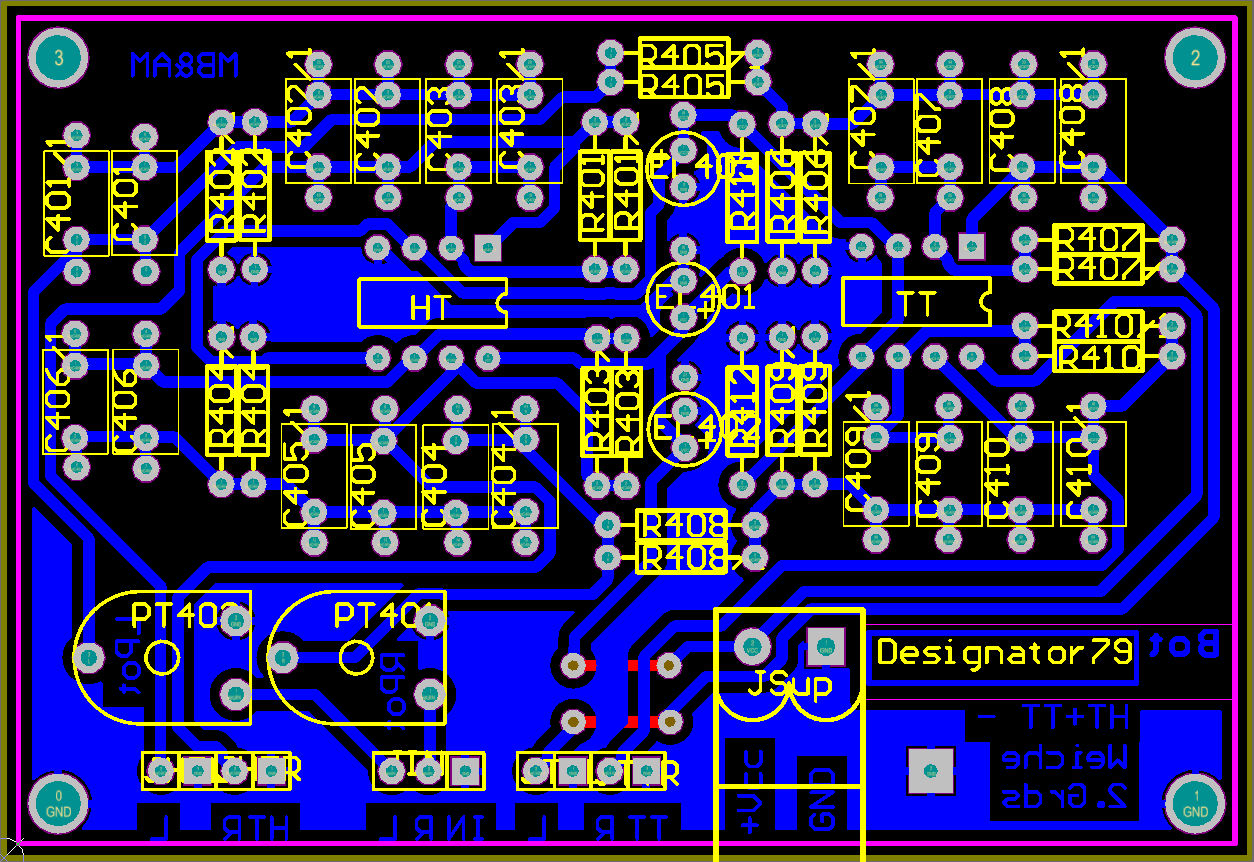
\includegraphics[width=1\textwidth]{img/Print4/4_TTuHTWeiche-PCB.PNG}
	\caption{Tieftöner- und Hochtönerweichen - PCB}
	\label {fig:4.2.5.1}
\end{figure}



